\documentclass[12pt,ngerman,parskip=half]{scrartcl}
\usepackage{babel}

\makeatletter % Mach das @ zu einem normalen Zeichen
\newcommand{\avg}{\mathop{\operator@font avg}}
\makeatother

\usepackage{amsmath,esvect, amsfonts}
\usepackage[standard,thmmarks]{ntheorem}
\usepackage{tikz}
\usetikzlibrary{arrows.meta}

\usepackage{hyperref}
\hypersetup{
    bookmarks=true,                     % show bookmarks bar
    unicode=false,                      % non - Latin characters in Acrobat’s bookmarks
    pdftoolbar=true,                        % show Acrobat’s toolbar
    pdfmenubar=true,                        % show Acrobat’s menu
    pdffitwindow=false,                 % window fit to page when opened
    pdfstartview={FitH},                    % fits the width of the page to the window
    pdftitle={My title},                        % title
    pdfauthor={Author},                 % author
    pdfsubject={Subject},                   % subject of the document
    pdfcreator={Creator},                   % creator of the document
    pdfproducer={Producer},             % producer of the document
    pdfkeywords={keyword1, key2, key3},   % list of keywords
    pdfnewwindow=true,                  % links in new window
    colorlinks=true,                        % false: boxed links; true: colored links
    linkcolor=blue,                          % color of internal links
    filecolor=cyan,                     % color of file links
    citecolor=green,                     % color of file links
    urlcolor=magenta                        % color of external links
}
\begin{document}

\listtheorems{theorem,}

\section{Wie man's besser nicht macht - \TeX\ Syntax}

$$ a^2 + b^2 = c^2 $$

Damit Ihr indess erkennt, woher dieser ganze Irrthum gekommen ist, und weshalb man die Lust anklagt und den $a^2 + b^2 = c^2$ Schmerz lobet, so will ich Euch Alles eröffnen und auseinander setzen, was jener Begründer der Wahrheit und gleichsam Baumeister des glücklichen Lebens selbst darüber gesagt hat. 

\section{Wie man's besser macht - \LaTeX\ Syntax}

Eckige Klammern für abgesetzte Formeln ohne Nummer und runde Klammern für Mathe im Fließtext.

\[ a^2 + b^2 = c^2 \]

Ebenso werde der Schmerz als solcher von Niemand geliebt, gesucht und verlangt, sondern weil mitunter solche Zeiten eintreten, dass man mittelst Arbeiten und Schmerzen \( a^2 + b^2 = c^2 \) eine grosse Lust sich zu verschaften suchen müsse. Um hier gleich bei dem Einfachsten stehen zu bleiben, so würde Niemand von uns anstrengende körperliche Übungen vornehmen, wenn er nicht einen Vortheil davon erwartete. 

\begin{equation}\label{eq:pythagoras}
-\frac{p}{2} \pm \sqrt{ \left(\frac{p}{2}\right)^2 -q }
\end{equation}

Siehe Gleichung \ref{eq:pythagoras}

Wer dürfte aber wohl Den tadeln, der nach einer Lust verlangt, welcher keine Unannehmlichkeit folgt, oder der einem Schmerze ausweicht, aus dem keine Lust hervorgeht?

\begin{equation}
\sum_{i=1}^{\infty} \sqrt[2\,]{i\times \prod_{x=\sum_{i=1}^{\infty}} \pi \cdot \alpha \beta \gamma 
\frac{\frac{1}{2}}{\frac{3}{4}}
}
\end{equation}

\begin{equation}
\overbrace{a^2+b^2}^3 = \underbrace{c^2 + d^2}_4
\end{equation}

\begin{equation}
\sin \beta \cos \tan \alpha \avg \gamma
\end{equation}

\begin{eqnarray} % LaTeX, besser nutzt man AMSmath
y &=& d \\
y &=& c_x +d \\
\sin x &=& \cos x \times y + \alpha - \beta
\end{eqnarray}

\begin{eqnarray*} % LaTeX, besser nutzt man aber ams
y &=& d \\
y &=& c_x +d \\
\sin x &=& \cos x \times y + \alpha - \beta
\end{eqnarray*}

\[
\begin{array}{lcr} % LaTeX
y &=& d \\
y &=& c_x +d \\
\sin x &=& \cos x \times y + \alpha - \beta
\end{array}
\]

\[ % LaTeX 
\bordermatrix{
   & 1 & 2 & 3 \cr
1 & 4 & 2 & 156 \cr
2 & 5 & 33 & 56 \cr
3 & 6 & 2 & 88 \cr
}
\]

\section{AMSmath}

\begin{align} % mit Nummern 
a &= c \cdot x \\
a &= c \cdot \tanh z + \sum_{i=1}^{1000} t
\end{align}

\begin{align*} % ohne Nummern 
a &= c \cdot x \\
a &= c \cdot \tanh z + \sum_{i=1}^{1000} t
\end{align*}

\begin{alignat}{3}
a &= c \cdot x &= x\times y \leq 567 \\
a &= c \cdot \tanh z + \alpha\omega &= \sum_{i=1}^{1000} t
\end{alignat}

\begin{alignat*}{3}
a &= c \cdot x &= x\times y \leq 567 \\
a &= c \cdot \tanh z + \alpha\omega &= \sum_{i=1}^{1000} t
\end{alignat*}


\[% Version ohne Klammern
\begin{matrix} 
1 & 0 & 0 \\ 
0 & 1 & 0 \\ 
0 & 0 & 1 \\ 
\end{matrix}
\]


\[% mit runden Klammern (parentheses)
\begin{pmatrix} 
1 & 0 & 0 \\ 
0 & 1 & 0 \\ 
0 & 0 & 1 \\ 
\end{pmatrix}
\]

\[% mit eckigen Klammern
\begin{bmatrix} 
1 & 0 & 0 \\ 
0 & 1 & 0 \\ 
0 & 0 & 1 \\ 
\end{bmatrix}
\]

\[% mit geschweiften Klammern
\begin{Bmatrix} 
1 & 0 & 0 \\ 
0 & 1 & 0 \\ 
0 & 0 & 1 \\ 
\end{Bmatrix}
\]


\[% mit senkrechten Strichen 
\begin{vmatrix} 
1 & 0 & 0 \\ 
0 & 1 & 0 \\ 
0 & 0 & 1 \\ 
\end{vmatrix}
\]

\[% mit doppelten senkrechten Strichen 
\det 
\begin{Vmatrix} 
\ddots  & 0 & \vdots \\ 
0 & \cdots & \dots \\ 
0 & 0 & 1 \\ 
\end{Vmatrix}
\text{ist eine Matrix}
\]

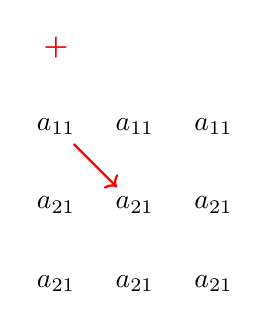
\begin{tikzpicture}
\node[red] at (0,1) (a11p)  {\bfseries+};

\node at (0,0) (a11)  {$a_{11}$};
\node at (0,-1) (a21)  {$a_{21}$};
\node at (0,-2) (a31)  {$a_{21}$};

\node at (1,0) (a12)  {$a_{11}$};
\node at (1,-1) (a22)  {$a_{21}$};
\node at (1,-2) (a32)  {$a_{21}$};

\node at (2,0) (a13)  {$a_{11}$};
\node at (2,-1) (a23)  {$a_{21}$};
\node at (2,-2) (a33)  {$a_{21}$};

\draw[red,thick,->] (a11) -- (a22);

\end{tikzpicture}

%Standard-Vektorpfeil skaliert nicht mit
\( \vec{a} \times \vec{def} \)

%esvect Paket laden für \vv-Befehl
\( \vv{a} \times \vv{def} \bigtriangleup \Omega  \)

\clearpage

\( ab \) % kein Abstand

\(a\,b \)

\(a\;b\)

\(a\quad b\)

\(a\qquad b\)

\(a \cup b \cap  c \subset d \supset e \)

\[ a \in N \forall  \]

\(  \mathbb{N} \)


\(  a_{1_{2_{3_4}}}   \) 


\begin{proof}
fsdfsd
\end{proof}

\begin{theorem}
fsdfsd
\end{theorem}

\begin{lemma}
fsdfsd
\end{lemma}

\begin{corollary}
fsdfsd
\end{corollary}

%https://tex.stackexchange.com/questions/270543/draw-a-graph-in-latex-with-tikz
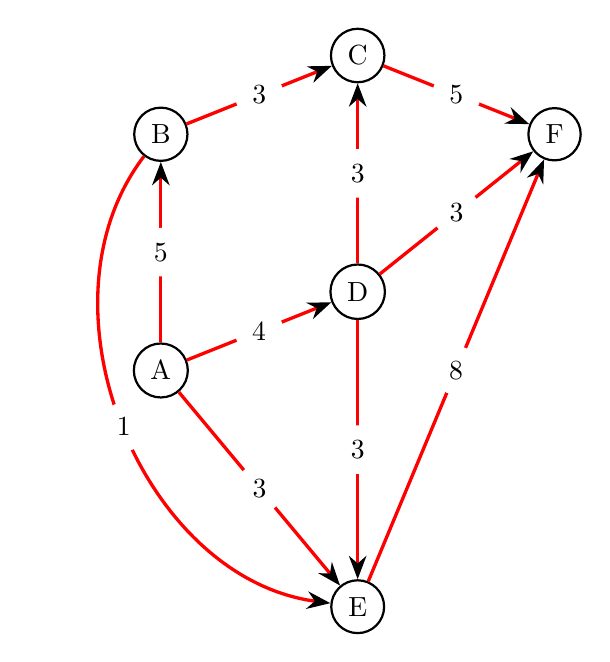
\begin{tikzpicture}
\begin{scope}[every node/.style={circle,thick,draw}]
    \node (A) at (0,0) {A};
    \node (B) at (0,3) {B};
    \node (C) at (2.5,4) {C};
    \node (D) at (2.5,1) {D};
    \node (E) at (2.5,-3) {E};
    \node (F) at (5,3) {F} ;
\end{scope}

\begin{scope}[>={Stealth[black]},
              every node/.style={fill=white,circle},
              every edge/.style={draw=red,very thick}]
    \path [->] (A) edge node {$5$} (B);
    \path [->] (B) edge node {$3$} (C);
    \path [->] (A) edge node {$4$} (D);
    \path [->] (D) edge node {$3$} (C);
    \path [->] (A) edge node {$3$} (E);
    \path [->] (D) edge node {$3$} (E);
    \path [->] (D) edge node {$3$} (F);
    \path [->] (C) edge node {$5$} (F);
    \path [->] (E) edge node {$8$} (F); 
    \path [->] (B) edge[bend right=60] node {$1$} (E); 
\end{scope}
\end{tikzpicture}

% https://tikz.dev/tikz-trees
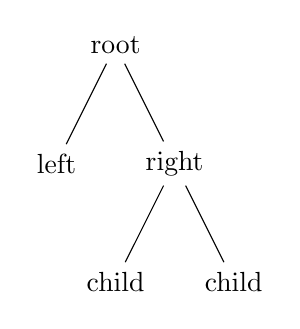
\begin{tikzpicture}
  \node {root}
    child {node {left}}
    child {node {right}
      child {node {child}}
      child {node {child}}
    };
\end{tikzpicture}

\end{document}